%GLOSSARY
%%%%%%%%%%%%%%%%%%%%%%%%%%%
%%%% Put the following at the top of each .tex file  %
\pagestyle{fancy}
\setcounter{page}{1}
\rhead{Glossary}
\lhead{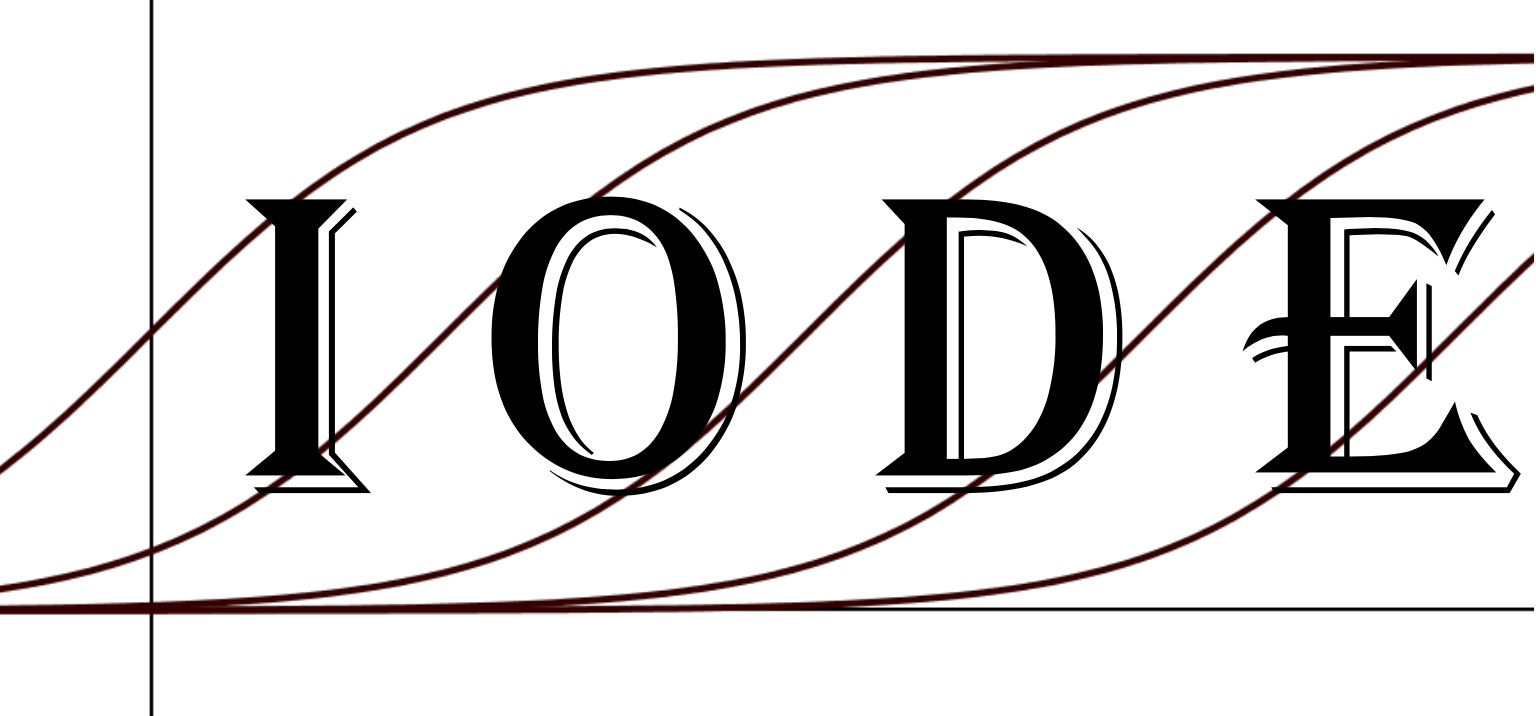
\includegraphics[width=1.25cm]{IODE-logo.png}}
\rfoot{Glossary Page \thepage}
\lfoot{}
\cfoot{}
\fancypagestyle{firstfooter}{\footskip = 50pt}
\renewcommand{\footrulewidth}{.4pt}
%%%%%%%%%%%%%%%%%%%%%%%%%%%
\vspace*{-20pt} \thispagestyle{firstfooter}
\pagebegin{Glossary for First Order Linear Differential Equations}
\begin{description}
\item[Analytic approach:] In this course, use have two analytic approaches \textbf{separation of variables} and the technique for \textbf{first order linear differential equations}. These approaches provide either general or particular solutions in algebraic or analytic form.
\item[Autonomous differential equation:] A differential equation where the derivative is dependent only on the dependent variable. For example $\frac{dy}{dt}=2y-3$ is autonomous, but $\frac{dy}{dt} = 2t -3$ is not autonomous. 
\item[Bifurcation diagram:] A plot of equilibrium solutions versus a parameter. Additionally, one can show phase lines on the graph which show whether equilibrium solutions are stable (attractor), unstable (repeller), or semi-stable (node).
\item[Bifurcation value:] A value of the parameter for which there is a change in the number or type of equilibrium solutions.
\item[Differential equation:] A differential equation is also known as a \textbf{rate of change equation}. An equation for an unknown function in terms of its derivative. Suppose $y = y(t)$ is some unknown function, then a differential equation, or rate of change equation, would express the rate of change, $\frac{dy}{dt}$, in terms of $y$ and/or $t$. \textbf{First order} differential equation contains only the first derivative. \textbf{Second order} differential equations contains derivatives up to the second derivative. An \textbf{ordinary differential equation (ODE)} is a differential equation whose derivatives pertain to only one variable, typically derivatives with respect to time. A \textbf{partial differential equation (PDE)} is a differential equation whose derivatives pertain to multiple variables.
\item[Equilibrium solution:] A constant function that satisfies a given differential equation. There are three types of equilibrium solutions for first order differential equations: attractors (stable), repellers (unstable), and nodes (semi-stable). 
\item[Euler's method:] Informally referred to as the ``tip to tail" method; this is a numerical method to find approximate solutions to a given differential equation.
\item[Exact solution:] A function that satisfies a given differential equation. That is, when the function is inserted into the differential equation a true statement results.
\item[Explicit solution:] The general solution has been written so that it is in the form $y(t) = e^{2t}$. Contrast this with \textbf{implicit solution}.
\item[First order linear differential equation:] A differential equation that can be written in the form $\frac{dy}{dt}+ g(t)y =r(t)$, where $g(t)$ and $r(t)$ are both continuous functions. This type of differential equation is solved using the analytic technique of \textbf{reverse product rule.}
\item[General solution:] An algebraic (sometimes referred to as analytic) representation of the family of functions that solve a given differential equation.
\item[Implicit solution:] The general solution has been left in a form that has not been (or cannot be) algebraically solved. For example, $y(t)^5 + y(t) = e^{2t}$.
\item[Initial condition or initial value:] A specific point through which the solution to a differential equation will pass. Usually expressed as $y_{t_0} = y_0$. For example, $y(0)=2$ (or $y(2)=6$) could be an initial condition that is then used to determine the \textbf{particular solution} from the \textbf{general solution}.
\item[Initial value problem (IVP):] A differential equation together with an initial condition (initial value) is called an Initial Value Problem (IVP).
\item[Integrating factor:] See \textbf{reverse product rule}.
\item[Numerical approach:] Provides numerical approximations to an initial value problem. One such method is \textbf{Euler's method}. Other methods include the Improved Euler's method and the \textbf{Runge-Kutta} method.
\item[Particular solution:] An algebraic (or analytic) representation of a specific function that solves the differential equation and contains a specified point, usually called the \textbf{initial value}. A differential equation together with an initial condition is referred to as an \textbf{initial value problem}.
\item[Qualitative / graphical approach] An approach to solving a differential equation that considers slopes and how the solution follows the slopes in a field.
\item[Reverse product rule:] A technique for solving a \textbf{first order linear differential equation} by introducing an unknown function $u$ to help ?undo? the product rule. $u$ is sometimes called an \textbf{integrating factor}.
\item[Runge-Kutta (RK4) method:] A fourth order method used in solving differential equations numerically. Contrast with \textbf{Euler's method} which is first order.
\item[Separable differential equation:] Differential equation that can be written in the form $\frac{dy}{dx}=f(y)g(x)$ and, when possible, solved using the analytic technique of \textbf{separation of variables}.
\item[Separation of variables:] An analytic technique to solve a differential equation of the form $\frac{dy}{dx}=f(y)g(x)$ by separating the variables (i.e., by rewriting it as $\frac{dy}{f(y)}=g(x)dx$) and integrating both sides if possible.
\item[Slope field:] A graphical representation of the slopes at many different points in a coordinate plane where each slope is determined by the derivative (rate of change) at any point in the plane. Slope fields can be used to sketch in graphs of solution functions. A curve that follows the slopes is the graphical analogue of inserting a function into the differential equation with the result giving a true statement.
\item[Uniqueness theorem:] Informally, the terms ``unique" or ``uniqueness" refers to whether or not two solution functions ever touch or cross each other. Refer to page 5.4 of the materials for the formal theorem.

\end{description}

\clearpage

\pagebegin{Glossary for Systems, Second Order, and Nonlinear DEs}
\begin{description}
\item[Characteristic equation:] A polynomial equation corresponding to a second order linear differential equation that is used to help find solutions.  
\item[Damping, Overdamped, Undamped:] Damping is the presence of a friction-like force in the system. Undamped is the lack of friction-like in the system. A system is called overdamped if the friction-like parameter exceeds a certain value determined by other parameters in the system.  
\item[Dependent (pertaining to linear algebraic equations):] A homogeneous system of two equations is dependent when it has infinitely many solutions.
\item[Eigensolution:] A straight line solution formed from an eigenvalue, eigenvector pair.
\item[Eigenvalue:] The value of the exponent associated with any straight line solution to a system of differential equations.
\item[Homogeneous differential equation:] The following second order differential equation, $P(t)\frac{d^2y}{dt^2}+Q(t)\frac{dy}{dt}+R(t)y=G(t)$, is homogenous when $G(t)=0$. The same holds true for higher order differential equations.
\item[Isocline:] An isocline is a set of points in the phase plane such that the slope of vectors is constant. Geometrically, these are the points where the vectors all have the same slope. Algebraically, we find isoclines by solving $\frac{dy}{dx} = c$. 
\item[Jacobian matrix:] A matrix that consists of all the first order partial derivatives of the differential equations in a system. When these partial derivatives are evaluated at a equilibrium solution, the Jacobian matrix linearizes a nonlinear system. 
\item[Linear system of differential equations:] A system in which the dependent variables appear in linear combinations, that is, they may be multiplied only by scalar quantities and combined only through addition and subtraction. For example, a two dimensional first order linear system of differential equations can be written as follows, where $a$, $b$, $c$, and $d$ are real numbers:
\begin{align*}
\frac{dx}{dt} &= ax + by \\
\frac{dy}{dt} &= cx + dy
\end{align*}
\item[Linearization:] The linearization, $L(h)$, of a function around a point of interest, $x^*$, is given by $L(h) \equiv f(x^*) + hf^\prime(x^*)$. The key feature of the linearization is that, when $x \approx x^*$, that is, $x = x^* + h$ for $h \approx 0$, then $f(x) \approx L(h)$.
\item[Method of undetermined coefficients:] This is a 3-step strategy to solve second order differential equations (1 - Find the general solution to the corresponding homogeneous equation; 2 - Find the particular solution to the nonhomogeneous equation, 3 - Add the previous results).
\item[Nonhomogenous differential equation:] A nonhomogeneous second order linear differential equation with constant coefficients has the form $y^{\prime\prime}+py^\prime+q=g(t)$, where $g(t)$ is nonzero. More generally, $P(t)\frac{d^2y}{dt^2}+Q(t)\frac{dy}{dt}+R(t)y=G(t)$ is a second order linear differential equation, where $G(t)$ is not zero. The same holds true for higher order differential equations.
\item[Nullcline:] The $x$-nullcline is a set of points in the phase plane such that $\frac{dx}{dt} = 0$. Geometrically, these are the points where the vectors point either straight up or straight down. Algebraically, we find the $x$-nullcline by solving $\frac{dx}{dt} = 0$. The $y$-nullcline is a set of points in the phase plane so that $\frac{dy}{dt} = 0$. Geometrically, these are the points where the vectors are horizontal, pointing either to the left or to the right. Algebraically, we find the $y$-nullcline by solving $\frac{dy}{dt} = 0$. The $x$-nullcline and $y$-nullcline are specific \textbf{isoclines}.
\item[Phase plane:] A plane where solutions and/or vectors for as system of differential equations can be represented in two dimensions. You often will see vectors and/or solutions represented.  
\item[Phase portrait:] Projection of the solution curves of a system like:
\begin{align*}
x^\prime &= f(x,y) \\
y^\prime &= g(x,y)
\end{align*}
into the $x-y$ (phase) plane. Usually the phase portrait include several representative solutions to help represent all the solutions.
\item[Vector field:] A vector field shows a selection of vectors with the correct slope with normalized length in a phase plane.

\end{description}